\documentclass{beamer}

\usepackage[italian]{babel} 
\usepackage[utf8x]{inputenc}
\usepackage{graphics}
\usepackage{default}
\usetheme[language=italian,
titlepagelogo=logoUnimi,
bullet=triangle,
pageofpages=of,
titleline=true,
color=blue,
bullet=cirlce,
assistantsupervisor=true
]{TorinoTh}

\title[Tesi di Laurea]{TECNICHE ONLINE PER L’INDIVIDUAZIONE DI SPAM IN UN WEB CRAWLER}
\institute{Università degli Studi di Milano}
\author{Antonio Luca}
\rel{Paolo Boldi}
\assistantsupervisor{Sebastiano Vigna}

\begin{document}
\begin{frame}
  \maketitle
\end{frame}
\begin{frame}
    \frametitle{Il fenomeno del web spam}
    \begin{block}<1->{Le cause}
    \begin{itemize}
    \item<1->Col crescere delle dimensioni del web, aumenta la difficoltà per i webmaster di far comparire una pagina tra i primi risultati di un motore di ricerca per una data query.
    \end{itemize}
    \end{block}
    \begin{block}<2->{Conseguenze}
    \begin{itemize}
        \item<1->Sviluppo di meccanismi di spam per tentare di ingannare gli algoritmi dei motori di ricerca al fine di ottenere un rank maggiore per una data pagina web. 
        \item<2->Sviluppo di tecniche di spam detection.
    \end{itemize}
    \end{block}
\end{frame}
\begin{frame}
  \frametitle{Obbiettivo della tesi}  
  Obbiettivo di questa tesi è stata l’analisi delle varie tecniche di spam detection descritte in letteratura al fine di valutarne il comportamento e vagliare la possibilità di utilizzo di tali tecniche online.
  \begin{block}<2->{Struttura della tesi}
  \begin{itemize}
  \item Classificazione delle varie tecniche di spam detection sulla base dei segnali utilizzati.
  \item Analisi online (durante la fase di crawling) degli algoritmi offline.
  \end{itemize}
  \end{block}
\end{frame}
 \begin{frame}
     \frametitle{Tecniche di spam detection}
     \begin{block}<2->{Classificazione}
     \begin{itemize}
     \item<3->Tecniche basate sul contenuto;	
     \item<4->Tecniche basate sul grafo del web;
     \item<5->Tecniche basate su segnali eterogenei.
     \end{itemize}
     \end{block}
 \end{frame}
\begin{frame}
    \frametitle{Tecniche basate sul contenuto}
    Un metodo per identificare lo spam basandosi sul contenuto di una pagina web è  quello di analizzare alcune feature delle pagine spam e confrontarle con le medesime feature delle pagine non spam al fine di ottenere dei valori con cui stimare la natura della pagina web.
    \begin{block}<2->{Esempi di feature}
    \begin{itemize}
    \item Numero di parole all'interno della pagina (Keyword Stuffing);
    \item Numero di parole all'interno dei titoli delle pagine;
    \item Lunghezza media delle parole all'interno delle pagine;
    \item Lunghezza del testo all'interno dell'elemento \(<a>\);
    \item Frazione di contenuto visibile;
    \end{itemize}
    \end{block}
\end{frame}
% \begin{frame}
%     \frametitle{Feature: Numero di parole nel body}
%   \begin{center}
%   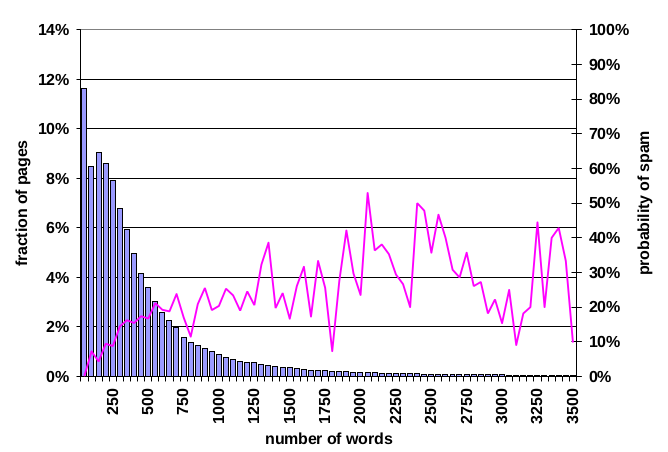
\includegraphics[width=8cm]{immagini/contenuto/fetterly3}
%   \end{center}
% \end{frame}
% \begin{frame}
%  \frametitle{Feature: Numero di parole nel titolo}
%   \begin{center}
%   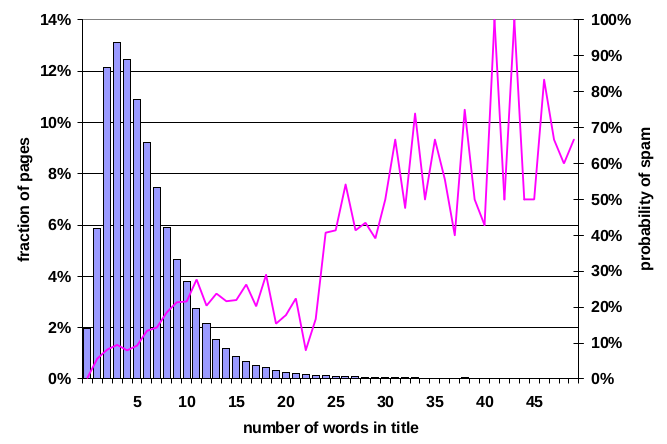
\includegraphics[width=8cm]{immagini/contenuto/fetterly4}
%   \end{center}
% \end{frame}
%\begin{frame}
%    \frametitle{Tecniche basate sul contenuto - 2}
%    \begin{itemize}
%     \item Viene utilizzata la \textit{Kullback-Leibler Divergence} (KLD) per misurare la divergenze tra le distribuzioni di probabilità dei termini	di pagine web, applicandola a unità di testo della pagina di partenza e di quella linkata
%     \item La Kullback-Leibler (KL) è una misura  asimmetrica della divergenza che misura quanto male una distribuzione di probabilità \(M_q\) riesce a modellare \(M_d\)
%     \begin{equation}
%KLD(T_1||T_2) = \sum_{t \in T_1} P_{T_1}(t) \log \frac{P_{T_1}(t)}{P_{T_2}(t)}
%\label{eqn:kld}
%     \end{equation}
%\end{itemize}
%\end{frame}
%\begin{frame}
%  \frametitle{KLD: Tipo di sorgenti}
%  \begin{block}<2->{Pagina di Partenza}
%  \begin{itemize}
%      \item testo delle ancore  
%   \item testo intorno alle ancore
%   \item termini nell'URL
%  \end{itemize}
%  \end{block}
%  \begin{block}<3->{Pagina di Arrivo}
%  \begin{itemize}
%   \item titolo della pagina  
%   \item contenuto della pagina
%   \item meta tag
%  \end{itemize}
%  \end{block}
%\end{frame}
%\begin{frame}
%  \frametitle{KLD: Uso delle sorgenti}
%  \begin{block}{Combinazione}
%  \begin{itemize}
%      \item testo delle ancore - contenuto  
%      \item testo vicino alle ancore - contenuto
%      \item termini nell’URL - contenuto
%      \item testo delle ancore - titolo
%      \item testo intorno alle ancore - titolo
%      \item termini nell’URL - titolo
%      \item titolo - contenuto
%      \item metatag
%  \end{itemize}
%  \end{block}
%\end{frame}
\begin{frame}
  \frametitle{Tecniche basate sul grafo}
  \begin{block}{Tecniche base}
  \begin{itemize}
  \item TrustRank
  \item Anti-trust Rank
% \item Spam mass
  \end{itemize}
  \end{block}
  \begin{block}<2->{}
  Utilizzano una versione personalizzata di PageRank:
  \begin{equation}
   \alpha G + (1-\alpha)\textbf{1}v^t
   \label{eqn:pagerank}
  \end{equation}
  \end{block}
  \end{frame}
\begin{frame}
  \frametitle{TrustRank}
  TrustRank tenta di assegnare un valore di rank maggiore alle pagine non spam rispetto alle pagine spam.
  \begin{block}<2->{Assunzione}
  \begin{itemize}
   \item Per determinare le pagine non spam viene fatta un’assunzione empirica chiamata isolazione approssimata dell’insieme delle pagine buone, la quale afferma che le pagine non spam raramente punteranno a delle pagine spam.
   \item Gli sviluppatori di pagine web non spam non hanno interesse nel linkare pagine spam (a meno che vengano “ingannati” tramite l’uso di tecniche come honeypot).
  \end{itemize}
  \end{block}
\end{frame}
\begin{frame}
  \frametitle{TrustRank}
  \begin{itemize}
   \item   TrustRank quindi è una versione personalizzata di PageRank dove il vettore di preferenza \(v\) non rappresenta una distribuzione uniforme su tutte le pagine del grafo \(G\) ma una distribuzione personalizzata dalle pagine del seedset di partenza.
$$
   \alpha G + (1-\alpha)\textbf{1}v^t
$$
  \end{itemize}
\end{frame}
\begin{frame}
  \frametitle{Anti-trust Rank}
  \begin{itemize}
   \item Parte dalla stessa intuizione dell'isolamento approssimato
   \item Utilizza un seedset iniziale composto da pagine spam
   \item Assume che una pagina spam (conosciuta) sia linkata solo da un'altra pagina spam 
   \item Come per TrustRank, utilizza Pagerank personalizzato sul grafo trasposto (prendendo in considerazioni i link in entrata)
   \item Assegna un rank maggiore alle pagine spam
  \end{itemize}
\end{frame}
%\begin{frame}
%  \frametitle{Spam mass}
%  \begin{itemize}
%   \item Per riconoscere una spam farm si parte dal presupposto che i nodi della spam farm hanno dei link uscenti verso delle pagine target \(t\) per aumentarne il rank
%   \item Spam mass è una misura che valuta l'impatto dello spam sul rank di una pagina
%   \item Vengono assegnati due valori: PageRank e Spam mass
%  \end{itemize}
%\end{frame}
% \begin{frame}
%   \frametitle{Determinazione della spam farm}
%   Partendo da un insieme \(\tilde{(V)}^+\) composto da pagine non spam conosciute
%    \begin{block}<2->{Si calcolano due misure}
%    \begin{itemize}
%     \item Spam mass assoluta: \(\tilde{M}_x=p_x-p'_x\)
%      \item Spam mass relativa:  \(\tilde{m}_x=(p_x-p'_x)/p_x=1-p'_x/px\)
%    \end{itemize}
%    dove \(p\) è il \textit{pagerank} dei nodi basato su una distribuzione uniforme mentre \(p'\) è \textit{pagerank} basato sull'insieme \(\tilde{(V)}^+\).
%    
%    Viene usato un valore di soglia per determinare se una pagina è parte di una spam farm.
%    \end{block}
% \end{frame}
\begin{frame}
  \frametitle{Tecniche eterogenee: Header HTTP}
\begin{itemize}
 \item Questo metodo utilizza le informazioni racchiuse all’interno degli header HTTP per determinare le pagine spam
 \item Può essere usato come supporto ad altri metodi descritti in precedenza e può essere utilizzato in modo dinamico durante la fase di download delle pagine
\end{itemize}
\begin{block}<2->{Funzionamento}
 \begin{itemize}
  \item Dopo aver effettuato la richiesta HTTP al server di una pagina vengono interpretati solo gli header della riposta HTTP
  \item Successivamente viene azionato un classificatore per valutare gli header come spam o non spam
  \item Se gli header vengono classificati come non spam allora si continua con la lettura del resto della pagina.
 \end{itemize}
\end{block}
\end{frame}
% \begin{frame}
%   \frametitle{Header HTTP - Esempio}
%   Analizzando i valori dei campi degli header HTTP si nota che alcuni di essi sono più frequenti nelle pagine spam invece delle pagine non spam
% \begin{center}
%  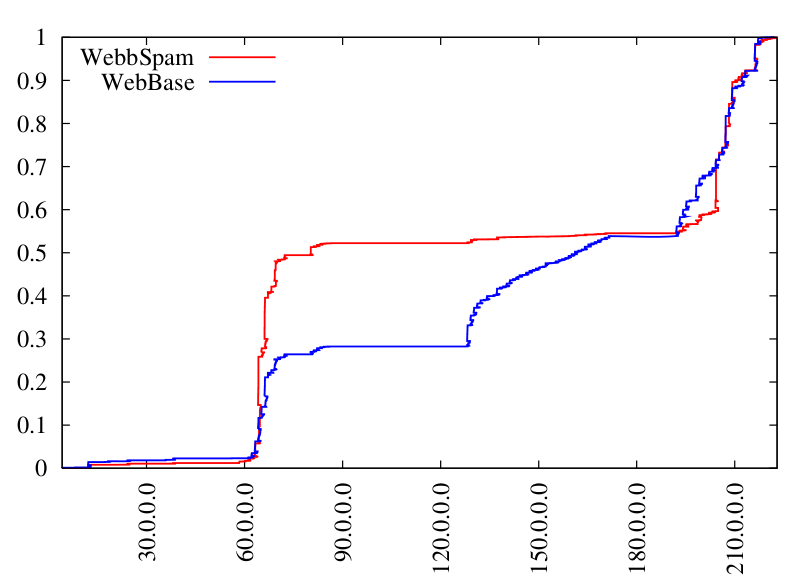
\includegraphics[width=6cm]{immagini/altre/webb}
% \end{center}
% \end{frame}
\begin{frame}
  \frametitle{Esperimenti}
  \begin{itemize}
   \item Si è scelto di valutare l’efficacia di due algoritmi link based offline (TrustRank e Anti-trust Rank) durante l’operazione di crawling ovvero in modo online.
   \item Razionale di tale analisi è stato la valutazione dell’operabilità di tali algoritmi durante l’esecuzione online e
il confronto delle prestazioni rispetto all’utilizzo convenzionale offline.
  \end{itemize}
  \begin{block}<2->{Nota}
   La simulazione della fase di crawling è stata fatta tramite una visita in ampiezza su grafo.
  \end{block}
\end{frame}
\begin{frame}
\frametitle{Esperimento 1 {\tiny(Confronto online/offline)}}
\begin{itemize}
 \item<1-> Calcolo della distanza, attraverso l’utilizzo della Tau di Kendall \(\tau_t\), tra il vettore \(t\) di TrustRank ricavato sull’intero grafo \(G\) e il vettore \(t_i\) di TrustRank calcolato sul grafo temporaneo \(G_v\), ricavato ad ogni intervallo di nodi visitati lungo una visita in ampiezza \(v\) con nodo sorgente \(s\).
 \item<2-> Calcolo della distanza, attraverso l’utilizzo della Tau di Kendall \(\tau_a\), tra il vettore \(a\) di Anti-trust Rank ricavato sull’intero grafo \(G\) e il vettore \(a_i\) di Anti-trust Rank calcolato sul grafo temporaneo \(G_v\), ricavato ad ogni intervallo di nodi visitati lungo una visita in ampiezza \(v\) con nodo sorgente \(s\).
\end{itemize}
\end{frame}
\begin{frame}
\frametitle{Esperimento 1 {\tiny(Confronto online/offline)}: Grafici}
\begin{center}
 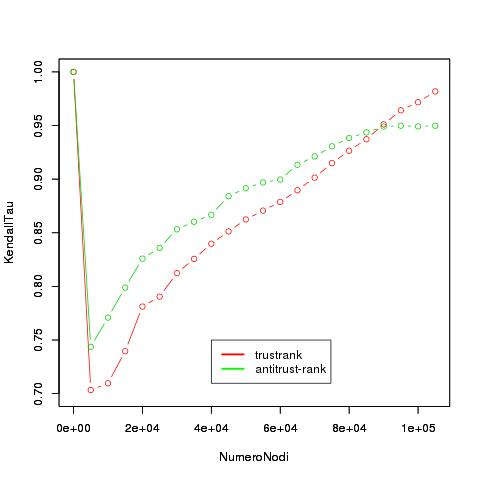
\includegraphics[height=6cm]{immagini/test1/coplotTrustAnti_62}
\end{center}
\end{frame}
%\begin{frame}
%\frametitle{Test 1: Risultati}
%\begin{itemize}
% \item<1-> Il comportamento tra \(\tau_{t}\) e \(\tau_{a}\) indica che TrustRank online è meno efficace di Anti-trust Rank nell'approssimare il comportamento offline. 
% \item<2-> Perciò tra questi due algoritmi quello che si adatta meglio nell'utilizzo in modalità online è Anti-trust rank perché tende ad approssimare fin da subito il comportamento offline. 
%\end{itemize}
%\end{frame}
\begin{frame}
\frametitle{Esperimento 2 {\tiny(Confronto online/offline parziale)}}
  \begin{itemize}
   \item<1-> Calcolo della distanza, attraverso l’utilizzo della Tau di Kendall \(\tau_t\), tra il vettore \(t\) di TrustRank ricavato sull’intero grafo \(G\) e il vettore \(t_i\) di TrustRank calcolato sul grafo temporaneo \(G_v\), prendendo in considerazione i soli nodi spam.
   \item<2-> Calcolo della distanza, attraverso l’utilizzo della Tau di Kendall \(\tau_a\), tra il vettore \(a\) di Anti-trust Rank ricavato sull’intero grafo \(G\) e il vettore \(a_i\) di Anti-trust Rank calcolato sul grafo temporaneo \(G_v\), prendendo in considerazione i soli nodi non spam.
  \end{itemize}
  \end{frame}
  \begin{frame}
\frametitle{Esperimento 2 {\tiny(Confronto online/offline parziale)}: Grafico TrustRank}
\begin{center}
 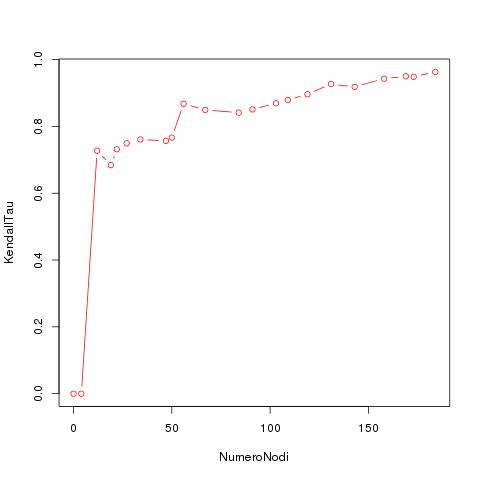
\includegraphics[height=6cm]{immagini/test2/trustrankBadNodesTestMode1_62}
\end{center}
\end{frame}
  \begin{frame}
\frametitle{Esperimento 2 {\tiny(Confronto online/offline parziale)}: Grafico Anti-trust Rank}
\begin{center}
 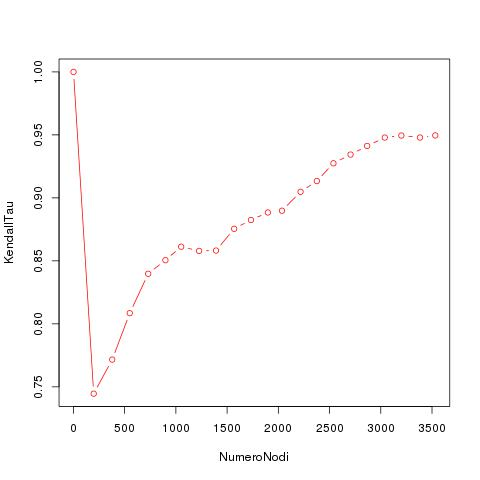
\includegraphics[height=6cm]{immagini/test2/antiTrustraktGoodNodesTestMode1_62}
\end{center}
\end{frame}
% \begin{frame}
% \frametitle{Test 2: Risultati}
% \begin{itemize}
%  \item<1-> Dai test si deduce che  Anti-trust Rank è più efficace di Trustrank in assoluto (vedi test 1) 
%  \item<2-> Trustrank è più efficace ad identificare i nodi spam
%  \end{itemize}
% \end{frame}
\begin{frame}
 \frametitle{Esperimento 3 {\tiny(Avversariale)}}
 Si è  simulata una situazione avversariale dove il seedset  utilizzato dagli algoritmi sia formato da nodi al limite del grafo \(G\).
\begin{center}
 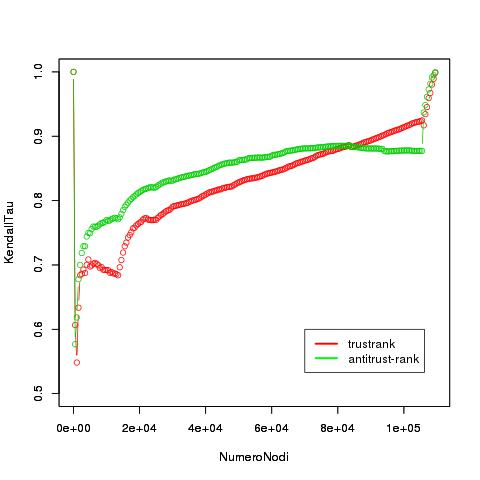
\includegraphics[height=6cm]{immagini/test3/coplotTrustAnti_Mode1_set3776_62}
\end{center}
\end{frame}
% \begin{frame}
% \frametitle{Test 3: Risultati}
% \begin{itemize}
%  \item<1-> Anti-trust Rank è meno dipendente dal vettore di preferenza che gli viene passato rispetto a Trustrank, almeno fino a quando il grafo temporaneo è al massimo l'80\% del grafo completo
%  \item<2-> Quindi anche se si usasse Anti-trust Rank in modalità online con un seedset poco pertinente questo riuscirebbe a produrre, fin dall'inizio del crawling, dei risultati molto vicini a quelli calcolati Anti-trust Rank sull'intero grafo con un altro seedset
%  \end{itemize}
% \end{frame}
\begin{frame}
\frametitle{Esperimento 4 {\tiny(Avversariale con \(\alpha\)=0.005)}}
Simile all'esperimento 3 ma il fattore di attenuazione \(\alpha\)  è impostato a 0.005.
   \begin{center}
 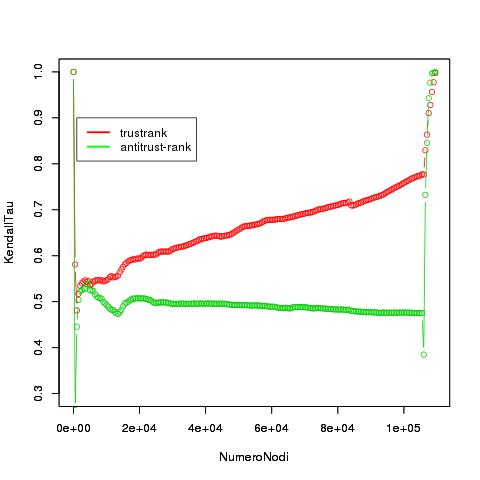
\includegraphics[height=6cm]{immagini/test4/coplotTrustAnti_Mode1_set3776_62_alpha0005}
\end{center}
\end{frame}
% \begin{frame}
% \frametitle{Test 4: Risultati}
% \begin{itemize}
%  \item<1-> TrustRank è meno dipendente dal fattore \(\alpha\) rispetto ad Anti-trust Rank
%  \end{itemize}
% \end{frame}
\begin{frame}
\frametitle{Esperimento 5 {\tiny(Separazione delle classi online)}}
\begin{itemize}
 \item Dal vettore di TrustRank,  calcolato sul grafo temporaneo, viene calcolata la differenza \(\Delta_t\) tra la media \(Mb_t\) dei valori di TrustRank dei nodi non spam e la media \(Ms_t\) dei valori di TrustRank dei nodi spam.
 \begin{equation}
 \Delta_t = Mb_t-Ms_t
\end{equation}
  \item Dal vettore di Anti-trust Rank,  calcolato sul grafo temporaneo, viene calcolata la differenza \(\Delta_a\) tra la media \(Mb_a\) dei valori di Anti-trust Rank dei nodi non spam e la media \(Ms_a\) dei valori di Anti-trust Rank dei nodi spam.
  \begin{equation}
 \Delta_a=Mb_a-Ms_a
\end{equation}
\end{itemize}
\end{frame}
\begin{frame}
\frametitle{Esperimento 5 {\tiny(Separazione delle classi online)}: TrustRank}
\begin{center}
 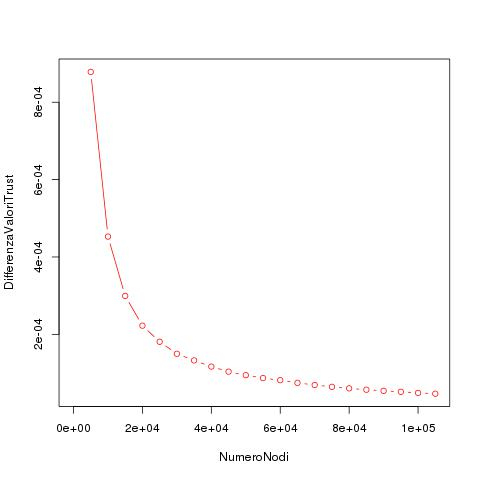
\includegraphics[height=6cm]{immagini/test5/averageTest_trust_62}
\end{center}
\end{frame}
% \begin{frame}
% \frametitle{Test 5: Risultati}
% \begin{itemize}
% \item<1-> Il risultato atteso è che durante la visita il calcolo di TrustRank discrimini in modo efficace i nodi non spam dai nodi spam e quindi che \(\Delta_t\) cresca durante la visita.
%  \item<2-> Ma i risultati del grafico indicano che all'inizio della visita la differenza \(\Delta_t\) ha un valore più alto rispetto alla differenza \(\Delta_t\) calcolata sul grafo temporaneo che si ottiene ai passi successivi della visita in ampiezza.
%  \item<3->Tale comportamento implica che la distanza tra i valori di TrustRank tra i nodi non spam e spam tende ad essere meno marcata tanto più il grafo temporaneo \(G_v\) su cui viene calcolato TrustRank cresce. 
%  \item<4-> Perciò invece di avere un andamento logaritmo i grafici sono contraddistinti da una parabola decrescente.
%  \end{itemize}
% \end{frame}
\begin{frame}
\frametitle{Esperimento 5 {\tiny(Separazione delle classi online)}: Anti-trust Rank}
\begin{center}
 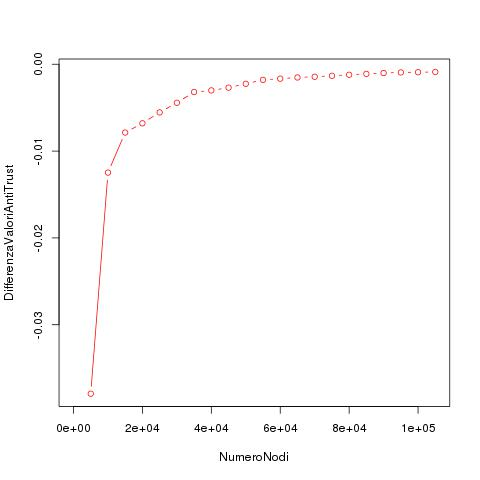
\includegraphics[height=6cm]{immagini/test5/averageTest_antitrust_62}
\end{center}
\end{frame}
% \begin{frame}
% \frametitle{Test 5: Risultati}
% \begin{itemize}
%  \item<1-> Anti-trust Rank calcolato verso la fine della visita dovrebbe restituire dei valori per i nodi non spam molto piccoli  e per i nodi spam dei valori molto alti. Si deduce quindi che alla fine della visita ,  \(Mb_a\) dovrebbe essere più piccola di \(Ms_a\) e di conseguenza che \(\Delta_a\) dovrebbe essere negativa . 
%  \item<2-> Anche in questo caso i risultati illustrati nei due grafici smentiscono il comportamento atteso in quanto il valore di \(\Delta_a\) aumenta con l'aumentare dei nodi del grafo temporaneo su cui viene calcolato Anti-trust Rank.
%  \end{itemize}
% \end{frame}
\begin{frame}
\frametitle{Esperimento 6 {\tiny(Separazione delle classi offline)}}
\begin{itemize}
 \item Il test è simile al esperimento 5 ma si utilizzano i valori ricavati da TrustRank e Anti-trust Rank calcolati sul grafo completo, invece di usare i valori temporanei di TrustRank e Anti-trust Rank per calcolare \(\Delta_t\) e \(\Delta_a\) durante la visita in ampiezza.
 \end{itemize}
\end{frame}
\begin{frame}
\frametitle{Esperimento 6 {\tiny(Separazione delle classi offline)}: TrustRank}
\begin{center}
 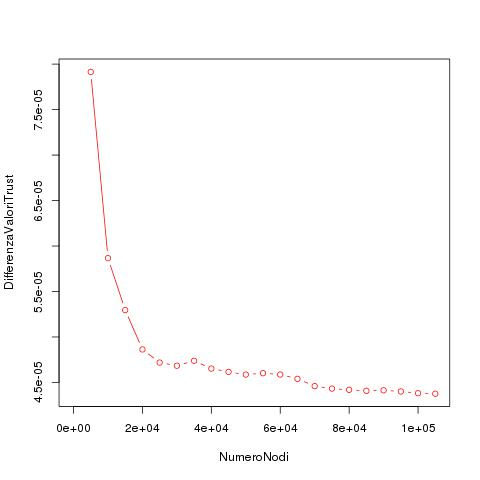
\includegraphics[height=6cm]{immagini/test6/averageCompleteTest_trust_62}
\end{center}
\end{frame}
% \begin{frame}
% \frametitle{Test 6: Risultati}
% \begin{itemize}
%  \item L'andamento del grafico giustifica i risultati ottenuti nel test numero 5  il quale ha un andamento molto simile.
%  \item Il range in cui variano i valori \(\Delta_t\), in questo test il range è di un ordine di grandezza più piccolo e quindi si deduce che la media dei valori di TrustRank del gruppo di nodi spam e la media TrustRank del gruppo di nodi non spam, contrariamente a quanto ci si aspetta, sono molto vicine. 
%  \item Perciò il test conferma che i risultati ottenuti nel test 5 dipendono dall'algoritmo di TrustRank.
%  \end{itemize}
% \end{frame}
\begin{frame}
\frametitle{Esperimento 6 {\tiny(Separazione delle classi offline)}: Anti-trust Rank}
\begin{center}
 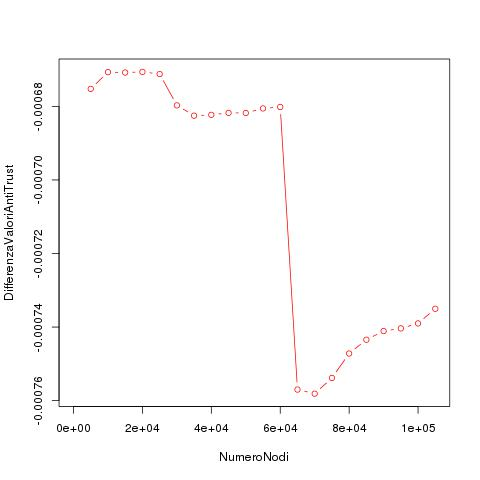
\includegraphics[height=6cm]{immagini/test6/averageCompleteTest_antitrust_62}
\end{center}
\end{frame}
% \begin{frame}
% \frametitle{Test 6: Risultati}
% \begin{itemize}
%  \item I risultati del grafico non seguano quelli del test 5
%  \item Ma dal momento che i  valori del grafico variano in un range molto piccolo possono confermare i risultati ottenuti nel test numero 5
%  \end{itemize}
% \end{frame}
\begin{frame}
 \frametitle{Conclusioni}
 \begin{itemize}
  \item TrustRank e Anti-trust Rank possono essere usati in modo online in quanto approssimano abbastanza bene il loro comportamento offline.
  \item Confrontando i due algoritmi si è evinto che Anti-trust Rank approssima meglio il comportamento offline, per quasi tutta la durata del crawling, e quindi è più indicato per essere usato in modo online.
   \end{itemize}
  \begin{block}{Sviluppi futuri}
    Sviluppo futuro di tale lavoro sarà la progettazione di un modulo di spam detection da inserire all’interno del web crawler BUbiNG.
  \end{block}
\end{frame}
\end{document}
